
\chapter{The Experiment}

\section{Large Hadron Collider}

The Large Hadron Collider (LHC) has a radius of approximately 27 kilometers. As of this writing, it is the largest machine ever constructed. The initial purpose of the LHC was to discover the Higgs boson, but it is capable of investigating a variety of other physics phenomena, such as dark matter, extra-dimensions, and heavy-ion physics. 

LHC is a hadron collider, meaning it is designed to collide particles made of quarks and gluons. The proton-proton, proton-Pb, and Pb-Pb collision energies are the largest ever probed experimentally.

\section{Compact Muon Solenoid}

The Compact Muon Solenoid (CMS) is a general-purpose particle detector located at Point-5 of the LHC. CMS was designed to precisely measure the momentum of muons. The titular superconducting solenoid magnet generates a 4 Tesla field. This field is homogeneous and parallel to the beam line close to the interaction point. The momentum of a muon is measured from how it deflects when moving through the magnetic field. 

\centerline{
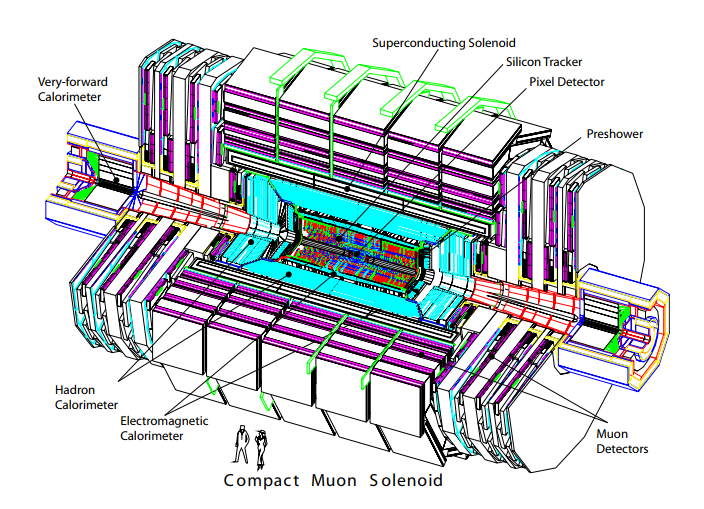
\includegraphics[width=5in]{Chapter3/importfigs/fromCMS_DesignPaper_perspective.png}
}

The central feature of the CMS apparatus is a superconducting solenoid of 6 m internal diameter, providing a magnetic field of 3.8 T. Within the solenoid volume are a silicon pixel and strip tracker, a lead tungsten crystal electromagnetic calorimeter (ECAL), and a brass and scintillator hadron calorimeter (HCAL), each composed of a barrel and two endcap sections. The silicon tracker measures charged particles within the pseudorapidity range $|\eta| < 2.5$ . It consists of 1440 silicon pixel and 15\,148 silicon strip detector modules and is located in the 3.8 $T$ field of the superconducting solenoid. For non-isolated particles of $1 < pt < 10 GeV$ and $|\eta| < 1.4$, the track resolutions are typically 1.5 percent in $pt$ and 25--90 (45--150)$\mu$ in the transverse (longitudinal) impact parameter~ cite (Chatrchyan:2014fea). 


The pseudorapidity coverage for the ECAL and HCAL detectors is $|\eta|< 3.0$. The ECAL provides coverage in the pseudorapidity range $y < $ 1.5 in the barrel region (EB) and 1.5 $< y <$ 3.0 in the two endcap regions (EE). The HCAL provides coverage for $y <$ 1.3 in the barrel region (HB) and 1.3 $< y< $ 3.0 in the two endcap regions (HE). The Hadronic Forward (HF) calorimeters ($3.0<|\eta| < 5.2 $) complement the coverage provided by the barrel and endcap detectors. The zero degree calorimeters (ZDCs) are two Cherenkov calorimeters composed of alternating layers of tungsten and quartz fibers, and situated between the two proton beam lines at above $|\eta|>8.3$ from the interaction point. The HF and ZDC systems each consist of two detectors on either side of the interaction point: $HF^{+-}$, and $ZDC^{+-}$, respectively. The CASTOR calorimeter is located at a distance of 14.2 m from the interaction point at a radial distance from the LHC beam of about 4 to 15 cm. This corresponds to a pseudorapidty coverage of -6.6 $< y <$ -5.2. A more detailed description of the CMS detector, together with a definition of the coordinate system used and the relevant kinematic variables, can be found in~ cite(Chatrchyan:2008aa).

\centerline{
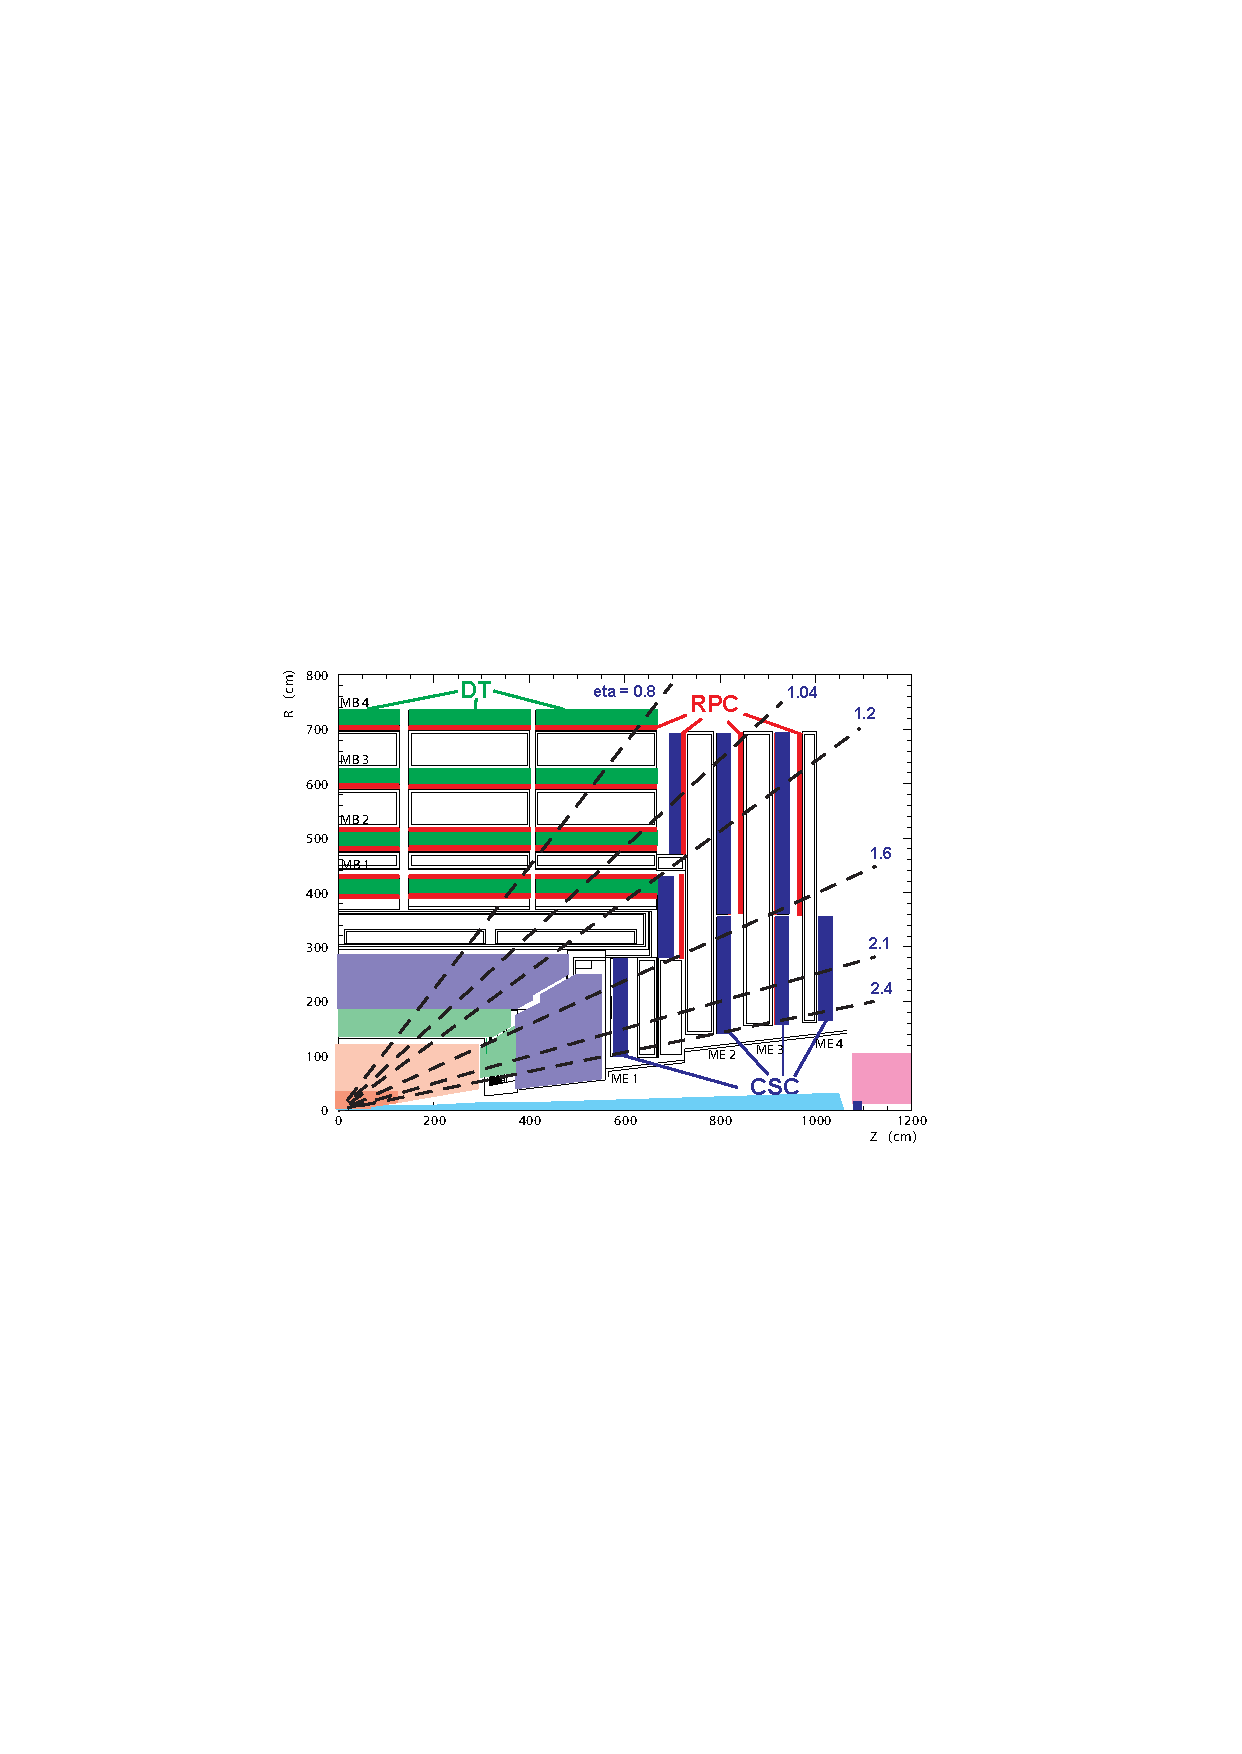
\includegraphics[width=5in]{Chapter3/importfigs/Figure_001-006.pdf}
}

\subsection{Inner Tracker}

The tracker measures the momentum of charged particles via their trajectory through a homogenous magnetic field. The tracker consists of two units, the pixel tracker and the strip tracker, both of which are made of silicon. A charged particle causes an electrical signal when passing through a silicon pixel or silicon microstrip. CMS reconstructs these electrical signals, taken at specific points of position and time, into tracks. These tracks are accurate to the 10 micrometers. The tracker is meant to have  a particle pass all the way through it, with only minimal effect particle's trajectory.

\subsubsection{Pixel Tracker}

Every silicon-pixel has a corresponding readout chip. The readout chips are soldered through the bump-bonding method. The readout chip amplifies signals from the pixel.

The pixel tracker is precise enough to distinguish the vertices of tracks originating from short-lived particles, such as bottomonia. 

\subsubsection{Strip Tracker}

\centerline{
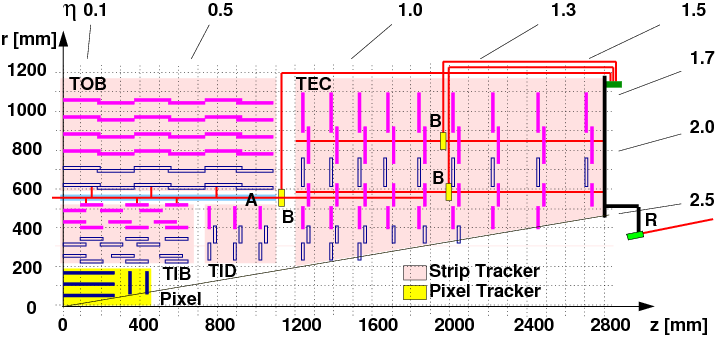
\includegraphics[width=5in]{Chapter3/importfigs/cms_cft_09_003_fig1.png}
}

\subsection{Electromagnetic Calorimeter}

The Electromagnetic Calorimeter (ECAL) is the dedicated CMS calorimeter for detecting electrons and photons. The calorimeter is comprised of lead tungstate ($PbWO_4$) crystals arranged in cylinder about the beam, including two endcaps. The granularity of these crystals gives the ECAL excellent energy resolution, angular resolution, and spatial resolution. The ECAL is hermetic and homogenous. The data readout is fast enough that CMS can trigger off signals in the ECAL.

\centerline{
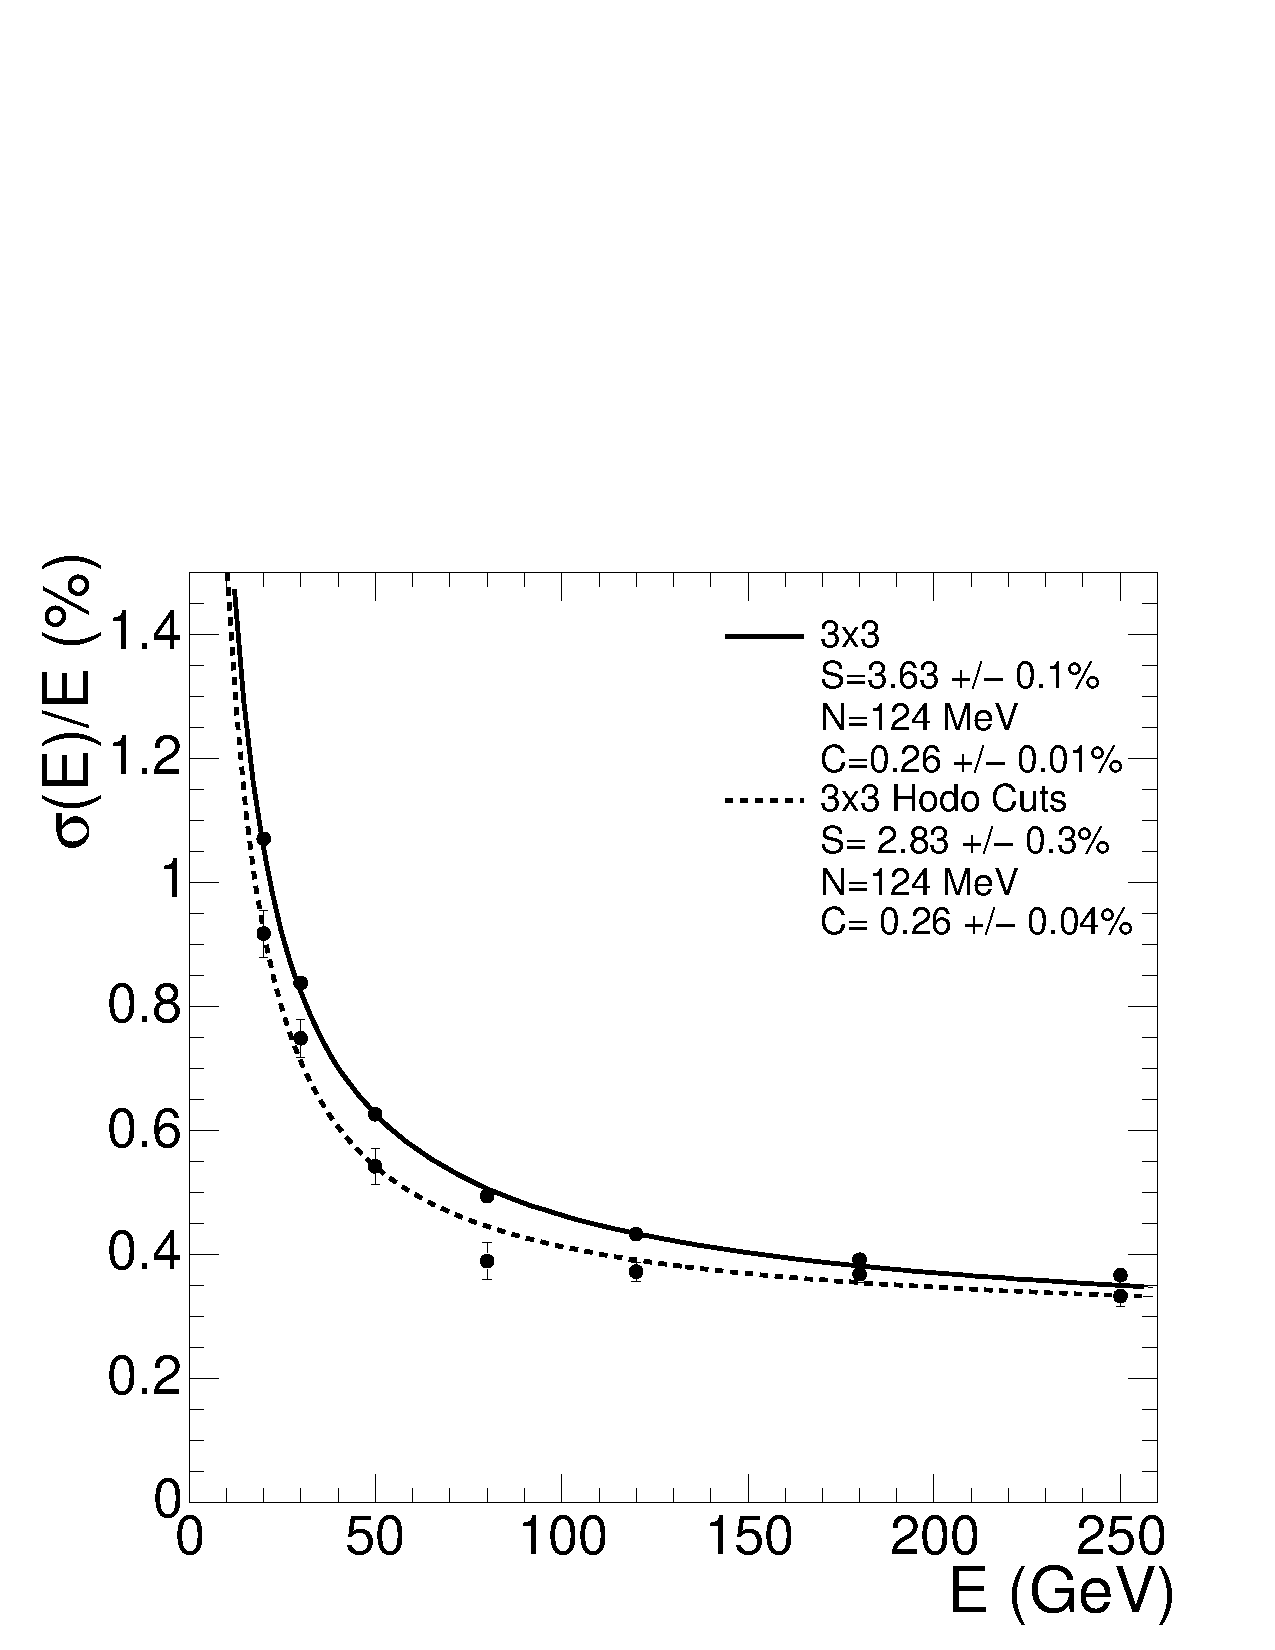
\includegraphics[width=5in]{Chapter3/importfigs/Figure_001-007.pdf}
}
 
\subsection{Hadronic Calorimeter}

The Hadronic Calorimeter (HCAL) has such a large acceptance that it can indirectly observe non-interacting particles such as neutrinos.

\centerline{
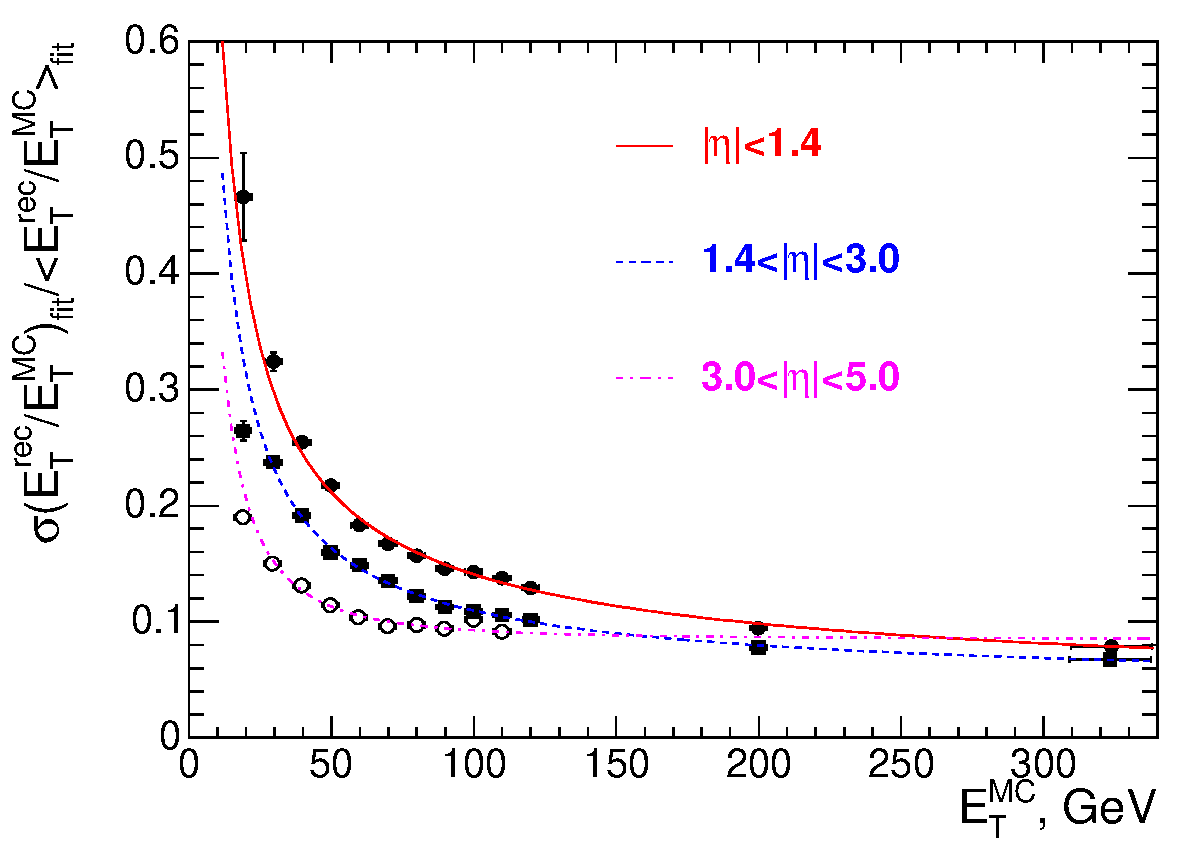
\includegraphics[width=5in]{Chapter3/importfigs/Figure_001-008.pdf}
}

\subsubsection{Hadronic Forward Calorimeters}

The Hadronic Forward Calorimeters (HF) absorbs the greatest portion of energy from collisions. As such it is designed for maximum radiative resistance.

\subsection{Muon Detector}



\subsection{Zero Degree Calorimeter}


\subsection{Particle Flow Algorithm}

\centerline{
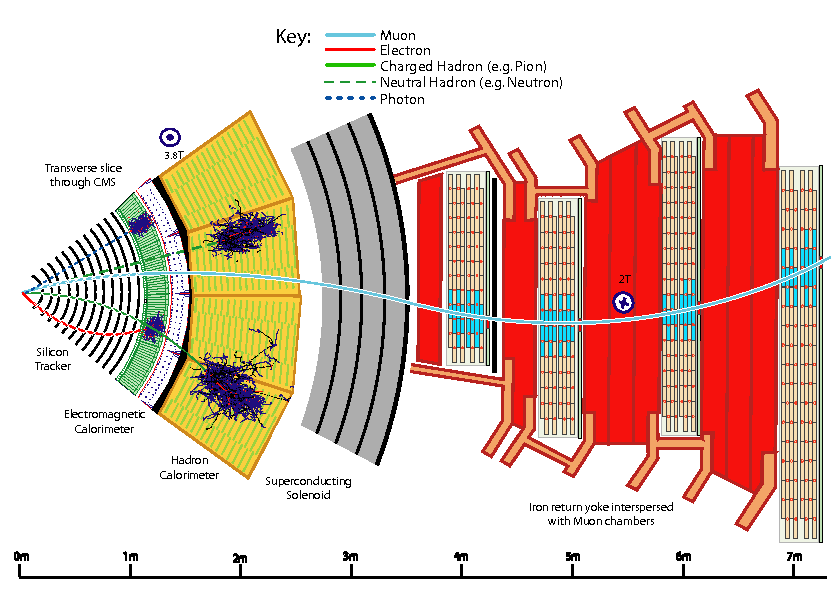
\includegraphics[width=5.5in]{Chapter3/importfigs/Figure_001.png}
}


\subsection{Luminosity}

One of the most important quantities measured by CMS is luminosity. Luminosity is necessary to convert the number of events detected, for a given channel, into a collision cross-section. Collision cross-sections are among the primary observables predicted by theoretical physics, specifically quantum field theory.

\subsubsection{van de Meer Scanning}

\subsection{Triggering}

CMS reconstruct events faster than they can be stored on hard-drives. To account for this phenomena -- pile-up -- CMS uses a two tiered triggering system. L1 triggers are always online, and for those events that pass the L1 triggers, the High Level Triggers (HLTs) will select which events are stored as data.